% \section{ Blockchain }
 Blockchain  o en español cadenas de bloques es una base de datos que puede ser utilizada de forma compartida 
con  usuarios que interactúan entre ellos de la manera peer-to-peer. La  Blockchain   almacena información y 
brinda la característica de ser inmutable y de estructurar  los datos en un orden secuencial \cite[]{retamal_Blockchain_2017}.

En ocasiones se confunde esta tecnología con el Bitcoin. Pero el Bitcoin es una moneda digital que utiliza la   Blockchain,
programada de una manera para obtener mayor grado de  seguridad y seudonimato en comparación a otras  Blockchain \cite[]{choo_Blockchain_2020}.


En el caso del Bitcoin los datos son públicos y pueden ser consultados en cualquier momento por cualquier 
usuario. 
Entonces la  Blockchain  es una base de datos compartida y descentralizada donde la modificación de las 
transacciones sea casi imposible, los datos (registros o transacciones) son 
almacenados dentro de un bloque y puede contener una o más transacciones. Para que los bloques sean agregados a la   Blockchain  
la mayoría de los nodos deben estar de acuerdo mediante algún tipo consenso o protocolo para validar la integridad de los bloques \cite[]{retamal_Blockchain_2017,choo_Blockchain_2020}.

Los nodos deben ejecutar algún tipo de consenso o protocolo para obtener un acuerdo  de que transacciones se 
almacenan en la  Blockchain,  para esto existen diferentes consensos, como la \gls{pow} \cite[]{retamal_Blockchain_2017}, \gls{pos} \cite[]{drescher_Blockchain_2017}, 
 \gls{poa}, según    el  algoritmo utilizado se requiere un nivel mayor o menor de  recursos y se obtiene 
más o menos seguridad. 
Estas bases de datos compartidas permiten que los registros almacenados no sean alterados. Para identificar 
quien es el propietario de los datos almacenados se le asigna una clave pública (identificadores visibles por
todos los nodos de la red) y una clave privada al usuario (utilizado para firmar las transacciones) \cite[]{retamal_Blockchain_2017}. 


\subsection{Funcionamiento de la Blockchain}
 La  Blockchain como se describió anteriormente, es una base de datos compartida
 por todos los usuarios de una red peer to peer. En  el caso de las  Blockchain públicas los datos
 pueden ser accedidos en cualquier momento y por cualquier usuario, la información añadida a la cadena de bloques pasa por un protocolo de consenso,
 o proceso para confirmar que la información que se pretende almacenar es correcta y cumple
 con las reglas definidas en la red \cite[]{retamal_Blockchain_2017,dannen_introducing_2017}.

Los nodos de la  Blockchain son pares iguales, en cada nodo se contiene la misma información con todas las transacciones realizadas
dentro de un bloque que contiene un número de transacciones (en el caso de Bitcoin cuenta con  alrededor de unas dos mil transacciones aproximadamente ) \cite[]{retamal_Blockchain_2017}.

Las llamadas transacciones, son los mensajes enviados desde una dirección a otra;  en ella 
 se almacenan datos como cantidades de una cierta moneda a gastar u otros, los que  dependen 
 de cómo  se hayan definido las reglas de la Blockchain. Pero por lo general, las transacciones transmiten una cantidad de una criptomoneda y adjuntan 
 datos extras. Ellas son enviadas a todos los nodos de la red en donde existe una competencia por cuál de los  nodos va almacenar primero el bloque con la 
 mayoría de las transacciones nuevas. La competencia se debe a que el nodo que resuelva un problema para poder agregar el bloque 
 recibe una recompensa con la criptomoneda nativa de su  Blockchain,  como en el caso de la prueba de trabajo, lo cual los nodos buscan
 obtener un hash para identificar al nuevo bloque  con ciertas características como ser iniciar el hash con una cantidad de ceros. De la manera que trabaja 
 Bitcoin, existen también otros tipos de competencias, ellas son denominadas algoritmos de consensos o protocolos de consensos.
Esto sirve para incentivar a los usuarios ser parte de la red, a mayor cantidad de nodos la red se vuelve más segura \cite[]{retamal_Blockchain_2017,nakamoto_bitcoin_2008,brys_cadena_2019}. 

El bloque nuevo se agrega a la base de datos apuntando al hash que representa el bloque anterior, de esta manera
cada bloque “apunta” hacia el bloque que le precede  pudiendo ir hasta la raíz y obtener todo el historial de las transacciones.
Los bloques almacenan información extra como el tiempo en el cual el bloque fue agregado a la cadena, la referencia hacia el bloque anterior, y otros 
datos dependiendo de las reglas que se han programado.
En la figura \ref{img:nakamoto_bloque}  se muestra la estructura de un bloque, donde  TX representa
las transacciones almacenadas en el bloque y el nonce (un numero que solo puede usarse una vez) es el número que hace que el hash del bloque cumpla con las reglas definidas para 
la competencia, por ejemplo, si se necesita que el hash del bloque inicie con tres ceros, los competidores (mineros) prueban diferentes valores, en el nonce
hasta hallar el hash que inicie con los tres ceros, esto no ocurre en todas las Blockchain, sino en las que cuentan con
el algoritmo de consenso prueba de trabajo \cite[]{drescher_Blockchain_2017,nakamoto_bitcoin_2008,kelly_investigation_2018,ethereum_org_transactions_2021}. 

\begin{figure}[H]
    \centering
    {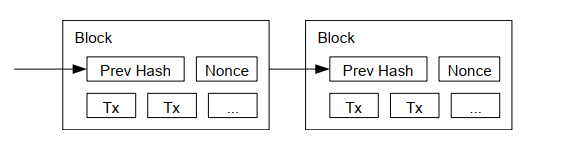
\includegraphics[scale=1]{nakamoto_bloque.png}}
    \caption{Estructura de una cadena de bloque genérica, imagen extraída del whitepaper de Nakamoto}
    \label{img:nakamoto_bloque}
\end{figure}


Las criptomonedas en la  Blockchain  son  definidas como una cadena de firmas digitales, donde cada dueño transfiere la moneda al próximo,
firmando digitalmente el hash de la transacción previa y la clave pública del destinatario. Entonces en la transacción se almacena el hash
de la transacción anterior más el mismo hash firmada por el emisor de la transacción, con lo cual se puede comprobar quien fue el emisor y también quien es el receptor.
Esta explicación se puede observar gráficamente en la figura \ref{img:nakamoto_transaccion} \cite[]{nakamoto_bitcoin_2008}. 

\begin{figure}[H]
    \centering
    {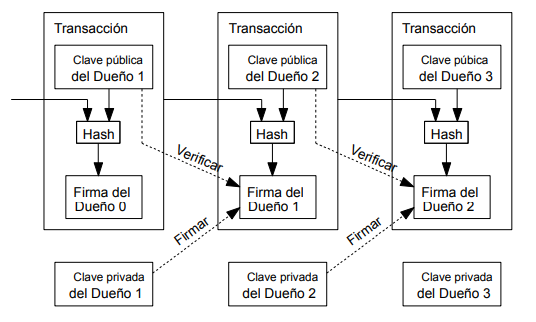
\includegraphics[scale=1]{nakamoto_transaccion.png}}
    \caption{Figura de una transacción, imagen extraída del whitepaper de Nakamoto}
    \label{img:nakamoto_transaccion}
\end{figure}

Con este protocolo cuando más grande es la red,  más difícil es poder modificar sus estados actuales, 
porque un nodo que modifique algún estado interno ya almacenado,
tiene que ser verificado para que todos los nodos los agreguen, si ven que no cumple con las reglas o los datos
no son los mismos que los demás nodos, se rechaza. 
Por ende, los datos almacenados en la Blockchain no pueden ser modificados, sin que todos los nodos lo modifiquen.
El autor de un ataque malicioso deberá tener el control de la mitad más un nodo para poder realizar sus acciones, pero esto resulta
muy costoso y a medida que la red crece, cada vez es más difícil realizarlo ya que el poder de cómputo de la red se vuelve más compleja \cite[]{nakamoto_bitcoin_2008,joaquin_lopez_lerida_economiBlockchain_2016}. 

Un minero es un nodo en la red que recopila transacciones y trabaja para organizarlas en bloques, 
 cada vez que reciben una transacción verifican si es correcta, y por el trabajo que realizan se les da una recompensa,
que son una pequeña comisión que es cobrada al emisor de la transacción y dependiendo del algoritmo de consenso, también se minan nuevas 
criptomoneda por bloque almacenado \cite[]{nakamoto_bitcoin_2008,joaquin_lopez_lerida_economiBlockchain_2016,preukschat_Blockchain_2018}.

\subsection{Características de una Blockchain}

En cuanto a las características más destacadas de la tecnología Blockchain se pueden mencionar a las siguientes \cite[]{torres_Blockchain_nodate}:

\begin{itemize}
    \item Seguridad y Privacidad: Los usuarios de la red pueden realizar transacciones libremente sin brindar ningun tipo de información personal
    simplemente firmando con su clave privada para verificar que le corresponde la clave pública. Pero la seguridad de las cadenas de bloques se da en la manera que
    se interconectan los bloques, donde cada uno de ellos referencia el bloque anteriormente generando un identificador único a partir del algoritmo de hash por lo tanto si algún dato del 
    bloque anterior es modificado el hash del siguiente  cambiará y 
    la cadena almacenada en el nodo no concordaría con los demás, por consecuencia es rechazada.  
    
    \item Trazabilidad: Es posible realizar un rastreo de todas las operaciones que fueron realizadas en una dirección específica, y también conocer 
  los recorridos de las transacciones que fueron ejecutadas, ya que todas ellas se encuentran enlazadas y 
    almacenadas en los nodos de la Blockchain. 

    \item Transparencia: En las  Blockchain públicas se conoce  su código fuente y el funcionamiento del sistema, esto permite 
    a los usuarios entender qué acciones están permitidas o no en el sistema y ver su funcionamiento real.
    
    \item Confianza: No es necesaria la confianza entre dos usuarios para realizar una transacción ya que el protocolo se encarga de realizar 
    el proceso.

    \end{itemize}

\subsection{Clases de Blockchain}
Existen las  Blockchain privadas, públicas e híbridas; las públicas son las nombradas a lo largo del documento y son las  Blockchain de Ethereum, EOS, Bitcoin. 
Las primeras  Blockchain fueron diseñadas para ser públicas. Cualquier individuo puede acceder sin ser usuario y leer las transacciones, cualquier 
persona o máquina puede convertirse en usuario y participar del protocolo,  todos los nodos son iguales, y seudónimas 
porque los dueños de las transacciones no necesitan brindar  datos personales, por lo cual se desconoce quíen es dueño de una dirección pero sí podrían ser
rastreables dado su carácter público \cite[]{preukschat_Blockchain_2018}.  

Las  Blockchains privadas también denominadas redes de permisos se caracterizan porque  pueden ser accedidas y utilizadas en algunas o todas las transacciones
por participantes de la red.  También por lo general cuentan con  distintos niveles de accesos según cómo se halla definido la Blockchain, por ejemplo, establecer 
diferentes tipos de roles.
Las redes privadas están compuestas en la mayoría de los casos de un número inferior de nodos, ya que la cantidad de participantes 
es limitada, pero la seguridad de la  Blockchain en general se caracteriza  porque a mayor números de nodos mayor seguridad \cite[]{torres_Blockchain_nodate}.

Al combinar las características de las  Blockchains públicas y privadas surgen las
 Blockchains híbridas. La  diferencia con las públicas y privadas  es 
en el protocolo de consenso. En lugar de ser un sistema abierto donde todos pueden validar los
bloques o uno cerrado donde una única entidad ejerce todo el control, nos encontramos con una
red donde el proceso de consenso es controlado por varias entidades, un grupo de nodos
funcionan como validadores de las transacciones \cite[]{torres_Blockchain_nodate}.

La ventaja de usar la  Blockchain es que todo los datos almacenados en ella son totalmente
accesibles, visibles, y permiten trazabilidad por lo tanto es  auditable \cite[]{drescher_Blockchain_2017}.
Absolutamente todo dato almacenado 
es válido, porque el protocolo asocia una dirección o address, con algún dato específico, el 
mismo puede ser manipulado (pero los cambios siguen almacenados) como lo permita el smart contract, el poseedor de algún dato
puede manejarlo según su voluntad cambiando estados del programas pero sin poder eliminar todo el historial de cambios realizados \cite[]{drescher_Blockchain_2017}.